%%__________________________________________________________________||
\section{Results and interpretation}
\label{sec:interpretation}

For a given category of events satisfying requirements on both \njet
and \nb, a likelihood model of the observations in all data samples is
used to obtain a consistent prediction of the SM backgrounds and to
test for the presence of a variety of signal models.% It is written as:

%\begin{align}
%  \label{likelihood}
%  L_{\njet,\,\nb} \; & = \; L_\text{SR} \times L_{\mu} \times
%  L_{\mu\mu} \times L_{\gamma} \, ; & (0 \leq \nb \leq 1) \\
%  L_{\njet,\,\nb} \; & = \; L_\text{SR} \times L_{\mu} \, , & (\nb
%  \geq 2)
%\end{align}

%where $L_\text{SR}$ describes the yields in each of the \scalht bins
%of the signal region where exactly \njet jets and \nb b-quark jets are
%required. 
In each bin of \scalht, the observation is modelled as a
Poisson-distributed variable about the sum of the SM expectation and a
potential signal contribution (assumed to be zero in the following
discussion). The contribution from multijet production is assumed
to be zero, based on the studies in Section~\ref{sec:multijet}. 
The SM expectation is related to the expected yields in
the \mj, \mmj, and \gj control samples via the transfer factors
derived from simulation. Likelihood functions %$L_\mu$,
%$L_{\mu\mu}$, and $L_\gamma$ 
describe the yields in the \scalht bins
of the \mj, \mmj, and \gj control samples in the same category of
\njet and \nb as the signal region. %For the category of events
%satisfying $\nb \geq 2$, only the \mj control sample is used in the
%likelihood to determine the total contribution from all non-multijet
%SM backgrounds in the signal region. 
The systematic uncertainties
%(4--26\%) 
associated with the transfer factors are accommodated in the
likelihood function by a nuisance parameter per transfer factor. The
measurements of these parameters are assumed to follow a log-normal
distribution.

%In order to test the compatibility of the observed yields with the
%expectations from only SM processes, the likelihood function is
%maximised over all fit parameters. For each of eight categories of
%events defined by requirements on \njet and \nb, the goodness-of-fit
%of the SM-only hypothesis is determined by considering simultaneously
%up to eleven bins in \scalht from the signal region and up to 30 bins
%from the three control samples. 
%Table~\ref{tab:fit-result} summarises the observed yields and fit
%results in bins of \scalht for events in the signal region categorised
%according to \njet and \nb. The uncertainties in the SM expectations,
%and p-values per event category, are determined from distributions
%that are built by generating pseudo-data from the likelihood function
%using the respective maximum-likelihood values of the nuisance
%parameters under the SM background-only hypothesis. 

%%No significant tension is observed between the signal and control
%%regions, which are well described by the SM-only hypothesis. 
%The category-level p-values are found to be uniformly distributed,
%with a minimum observed value of 0.17. The compatibility of the SM
%expectation and observed event count is also evaluated for each of the
%75 signal region bins. A profile likelihood ratio is used to determine
%a p-value and Z-score for each bin.
%%The pseudo-signal contribution is restricted to the relevant bin.
%% Twice the negative difference in the log likelihoods is distributed
%% according to a $\chi^2$ per degree of freedom, which is subsequently
%% converted into a pull (\ie Z-score) and a p-value. The pulls and
%% p-values are distributed as expected 
%The observed distributions of p-values and Z-scores are uniformly and
%normally distributed according to expectation, with the observed
%fluctuations in the positive tail of Z-score distribution occurring
%with a probability of not less than 0.5\%.
%%exhibiting a significance of, at most, 2.5 standard deviations.
%%A larger-than-expected number of bins with a pull of at least +1 is
%%observed, the probability for which is 4.4\% based on
%%pseudo-experiments.

The expected number of events from SM processes is determined from a
simultaneous fit to the signal region and up to three control
samples. The likelihood function is maximised over all fit parameters
under the SM-only hypothesis. \FIXME{Table of numbers here?} 
%Figure~\ref{fig:SMfithadronic} and Table~\ref{tab:fit-result} summarise
%the observed yields and expected event counts in bins of HT for events
%in the signal region categorised according to \njet and \nb. 
%
No significant tension is observed between the signal and control
regions, which are well described by the SM-only hypothesis.% The
%category-level p-values are found to be uniformly distributed, with a
%minimum observed value of 0.19. 
%yes, P-value is still correct

%\begin{table}[h!]
%  \caption{Observed event yields and expected SM-only event counts
%    with associated uncertainties in bins of \scalht for events in the
%    signal region that are categorised according to \njet and \nb.
%  }
%  \label{tab:fit-result}
%  \centering
%  \tiny
%  \begin{tabular}{ llllllllllllll }
%    \hline
%    \hline
%    \multicolumn{3}{c}{} & \multicolumn{11}{c}{\scalht (GeV)}                                                                                                                                                                                                                                            \\ 
%    \njet                & \nb      &        & 200--275              & 275--325             & 325--375             & 375--475             & 475--575             & 575--675             & 675--775             & 775--875             & 875--975             & 975--1075           & 1075--$\infty$      \\ 
%    \hline
%    2--3                 & $0$      & Data\T & $13090$              & $5331$               & $3354$               & $2326$               & $671$                & $206$                & $76$                 & $29$                 & $10$                 & $9$                 & $2$                 \\
%    2--3                 & $0$      & SM\B   & $13034^{+89}_{-117}$ & $5348^{+85}_{-67}$   & $3351^{+56}_{-50}$   & $2351^{+38}_{-45}$   & $655^{+14}_{-11}$    & $218^{+12}_{-17}$    & $68.5^{+4.9}_{-4.8}$ & $27.2^{+3.0}_{-3.0}$ & $10.4^{+1.5}_{-1.6}$ & $5.6^{+1.0}_{-1.0}$ & $4.3^{+0.7}_{-1.0}$ \\ 
%    2--3                 & $1$      & Data\T & $1733$               & $833$                & $527$                & $356$                & $90$                 & $31$                 & $6$                  & $4$                  & $1$                  & $0$                 & $1$                 \\
%    2--3                 & $1$      & SM\B   & $1711^{+37}_{-33}$   & $839^{+21}_{-25}$    & $526^{+20}_{-17}$    & $372^{+12}_{-14}$    & $90.6^{+5.1}_{-4.6}$ & $25.8^{+2.9}_{-2.6}$ & $8.7^{+0.8}_{-1.4}$  & $3.0^{+0.7}_{-0.6}$  & $2.2^{+0.8}_{-0.6}$  & $0.3^{+0.2}_{-0.1}$ & $0.2^{+0.1}_{-0.2}$ \\ 
%    2--3                 & $2$      & Data\T & $172$                & $116$                & $101$                & $55$                 & $16$                 & $9$                  & $0$                  & $0$                  & $0$                  & \multicolumn{2}{c}{}                      \\ 
%    2--3                 & $2$      & SM\B   & $184^{+5}_{-7}$      & $117^{+7}_{-5}$      & $99.4^{+5.4}_{-4.6}$ & $60.2^{+3.5}_{-3.8}$ & $12.4^{+1.2}_{-1.0}$ & $3.3^{+0.6}_{-0.5}$  & $0.7^{+0.2}_{-0.2}$  & $0.2^{+0.1}_{-0.1}$  & $0.1^{+0.0}_{-0.0}$  & \multicolumn{2}{c}{}                      \\
%    $\geq 4$             & $0$      & Data\T & $99$                 & $568$                & $408$                & $336$                & $211$                & $117$                & $38$                 & $13$                 & $9$                  & $4$                 & $6$                 \\
%    $\geq 4$             & $0$      & SM\B   & $104^{+6}_{-8}$      & $544^{+21}_{-18}$    & $407^{+18}_{-18}$    & $337^{+15}_{-10}$    & $202^{+10}_{-8}$     & $105^{+9}_{-7}$      & $42.5^{+4.5}_{-3.3}$ & $14.3^{+1.7}_{-2.5}$ & $7.5^{+1.4}_{-1.5}$  & $3.5^{+0.8}_{-0.8}$ & $3.4^{+1.0}_{-0.7}$ \\ 
%    $\geq 4$             & $1$      & Data\T & $38$                 & $195$                & $210$                & $159$                & $83$                 & $33$                 & $7$                  & $10$                 & $4$                  & $1$                 & $1$                 \\
%    $\geq 4$             & $1$      & SM\B   & $38.9^{+2.2}_{-3.7}$ & $206^{+12}_{-10}$    & $209^{+13}_{-10}$    & $157^{+9}_{-9}$      & $79.3^{+5.2}_{-4.7}$ & $29.4^{+3.8}_{-2.2}$ & $9.9^{+1.9}_{-1.3}$  & $6.2^{+1.2}_{-1.1}$  & $2.3^{+0.7}_{-0.7}$  & $0.9^{+0.3}_{-0.3}$ & $0.9^{+0.3}_{-0.4}$ \\ 
%    $\geq 4$             & $2$      & Data\T & $16$                 & $81$                 & $88$                 & $64$                 & $43$                 & $14$                 & $5$                  & $1$                  & $1$                  & \multicolumn{2}{c}{}                      \\ 
%    $\geq 4$             & $2$      & SM\B   & $12.5^{+1.0}_{-1.0}$ & $77.8^{+4.7}_{-4.6}$ & $90.2^{+9.0}_{-6.5}$ & $66.1^{+4.6}_{-4.8}$ & $36.3^{+3.4}_{-2.9}$ & $11.4^{+1.8}_{-1.9}$ & $3.9^{+0.8}_{-0.7}$  & $1.0^{+0.2}_{-0.3}$  & $0.7^{+0.1}_{-0.2}$  & \multicolumn{2}{c}{}                      \\ 
%    $\geq 4$             & $3$      & Data\T & $0$                  & $7$                  & $5$                  & $5$                  & $6$                  & $1$                  & $1$                  & $0$                  & $0$                  & \multicolumn{2}{c}{}                      \\ 
%    $\geq 4$             & $3$      & SM\B   & $1.1^{+0.2}_{-0.2}$  & $8.1^{+0.9}_{-0.9}$  & $9.9^{+1.5}_{-1.3}$  & $7.2^{+0.9}_{-0.7}$  & $4.1^{+0.6}_{-0.6}$  & $1.1^{+0.3}_{-0.3}$  & $0.4^{+0.1}_{-0.1}$  & $0.1^{+0.1}_{-0.0}$  & $0.1^{+0.0}_{-0.0}$  & \multicolumn{2}{c}{}                      \\ 
%    $\geq 4$             & $\geq 4$ & Data\T & $0$                  & $0$                  & $0$                  & $2$                  & \multicolumn{7}{c}{}                                                                                                                                         \\
%    $\geq 4$             & $\geq 4$ & SM\B   & $0.0^{+0.0}_{-0.0}$ & $0.1^{+0.1}_{-0.1}$  & $0.4^{+0.2}_{-0.3}$  & $0.4^{+0.2}_{-0.2}$  & \multicolumn{7}{c}{}                                                                                                                                         \\ 
%    2--3                 & $0$      & Data\T & $13310$               & $5404$               & $3580$               & $2475$               & $698$                & $224$                & $81$                 & $28$                 & $12$                 & $9$                 & $3$                 \\
%    2--3                 & $0$      & SM\T   & $13235^{+119}_{-101}$ & $5417^{+73}_{-62}$   & $3562^{+69}_{-48}$   & $2482^{+38}_{-40}$   & $689^{+15}_{-13}$    & $231^{+13}_{-10}$    & $72.2^{+5.2}_{-4.0}$ & $28.1^{+3.2}_{-3.0}$ & $11.2^{+1.4}_{-1.6}$ & $6.0^{+1.1}_{-0.9}$ & $3.7^{+0.9}_{-0.7}$ \\ 
%    2--3                 & $1$      & Data\T & $1802$                & $835$                & $597$                & $416$                & $97$                 & $29$                 & $7$                  & $4$                  & $1$                  & $0$                 & $0$                 \\
%    2--3                 & $1$      & SM\T   & $1743^{+32}_{-32}$    & $843^{+23}_{-26}$    & $580^{+23}_{-18}$    & $413^{+16}_{-14}$    & $102^{+5}_{-5}$      & $27.0^{+2.8}_{-2.9}$ & $9.1^{+1.2}_{-1.2}$  & $3.3^{+0.7}_{-0.7}$  & $2.3^{+0.7}_{-0.6}$  & $0.3^{+0.2}_{-0.1}$ & $0.2^{+0.1}_{-0.1}$ \\ 
%    2--3                 & $2$      & Data\T & $174$                 & $119$                & $117$                & $70$                 & $18$                 & $7$                  & $1$                  & $0$                  & $0$                  & \multicolumn{2}{c}{}                      \\ 
%    2--3                 & $2$      & SM\T   & $176^{+8}_{-6}$       & $115^{+6}_{-6}$      & $104^{+6}_{-5}$      & $68.1^{+4.7}_{-4.7}$ & $15.2^{+1.6}_{-1.5}$ & $3.3^{+0.5}_{-0.6}$  & $1.1^{+0.3}_{-0.3}$  & $0.2^{+0.1}_{-0.1}$  & $0.1^{+0.0}_{-0.0}$  & \multicolumn{2}{c}{}                      \\ 
%    $\geq 4$             & $0$      & Data\T & $103$                 & $590$                & $455$                & $391$                & $274$                & $149$                & $56$                 & $18$                 & $12$                 & $7$                 & $8$                 \\
%    $\geq 4$             & $0$      & SM\T   & $104^{+6}_{-8}$       & $567^{+21}_{-20}$    & $454^{+20}_{-19}$    & $397^{+14}_{-14}$    & $250^{+11}_{-10}$    & $134^{+10}_{-8}$     & $55.5^{+4.4}_{-4.1}$ & $19.2^{+2.5}_{-2.1}$ & $9.8^{+1.6}_{-1.4}$  & $4.6^{+1.0}_{-1.0}$ & $4.2^{+1.0}_{-0.9}$ \\ 
%    $\geq 4$             & $1$      & Data\T & $38$                  & $207$                & $250$                & $181$                & $108$                & $41$                 & $10$                 & $14$                 & $6$                  & $1$                 & $1$                 \\
%    $\geq 4$             & $1$      & SM\  & $104^{+6}_{-6}$      & $36.4^{+3.5}_{-3.3}$ & $14.2^{+1.8}_{-1.8}$ & $8.6^{+1.5}_{-1.4}$  & $3.9^{+0.9}_{-0.8}$  & $1.1^{+0.4}_{-0.3}$ & $1.2^{+0.4}_{-0.4}$ \\ 
%    $\geq 4$             & $2$      & Data\T & $17$                  & $82$                 & $95$                 & $86$                 & $48$                 &  & \multicolumn{2}{c}{}                      \\ 
%    $\geq 4$             & $3$      & SM\T   & $1.0^{+0.2}_{-0.2}$   & $8.2^{+0.8}_{-0.8}$  & $10.9^{+1.6}_{-1.5}$ & $8.2^{+1.1}_{-1.1}$  & $5.8^{+1.0}_{-0.8}$  & $2.2^{+0.6}_{-0.5}$  & $0.9^{+0.3}_{-0.2}$  & $0.2^{+0.1}_{-0.1}$  & $0.2^{+0.1}_{-0.1}$  & \multicolumn{2}{c}{}                      \\ 
%    $\geq 4$             & $\geq 4$ & Data\T & $0$                   & $ccurate and consistent prediction of the SM background,
%a simultaneous binned likelihood fit using information from all three
%data samples is performed. The fit maximizes the likelihood $L_\text{
%total} = L_\text{hadronic} \times L_{\mu+\text{jets}} \times L_{\gamma
%+ \text{jets}}$, where $L_\text{hadronic}$ characterizes
%$R_{\alpha_{\rm{T}}}$($\scalht$) in the hadronic sample with a single
%exponential function, $A\mathrm{e}^{-k \, H_\text{T}}$, to accommodate any
%QCD contamination and a constant, \scalht-independent contribution,
%$B$, to describe SM processes with genuine \met. The likelihoods
%$L_{\mu + \text{jets}}$ and $L_{\gamma+ \text{jets}}$ describe the
%\scalht-dependent yields in the $\mu$ + jets and $\gamma$ + jets
%samplebackgrounds, 

The results of this search are interpreted in terms of limits in the
parent sparticle and LSP mass parameter space of simplified
models~\cite{Alwall:2008ag, Alwall:2008va, sms} that represent the pair production of gluinos and their subsequent decays to four quarks 
and an LSP. Models in which the gluinos decay inclusively to all quark flavours, and models in which the decay is to four top and bottom quarks, respectively, are considered. 
%
% modes $\sTop
%\rightarrow{\rm c} \chiz_1$, $\sTop \rightarrow{\rm bf\bar{f'}}
%\chiz_1$, $\sTop \rightarrow {\rm b} \chipm_1$ fohe control samples. 
Only a subset of the event categories, chosen according to expected sensitivity, are used for
each interpretation.
%Table~\ref{tab:categories} specifies the event categories, defined in
%terms of \njet and \nb, used to provide interpretations in the
%different simplified models.

The event samples for the simplified models are generated 
%at leading order with %\PYTHIA6.4~\cite{pythia}. 
with \MADGRAPH V5~\cite{madgraph}.
Inclusive, process-dependent, NLO
calculations of SUSY production cross sections, with
next-to-leading-logarithmic (NLL) corrections, are obtained with the
program \PROSPINO~\cite{Beenakker:1996ch, PhysRevD.80.095004,
  PhysRevLett.102.111802, PhysRevD.80.095004, 1126-6708-2009-12-041,
  doi:10.1142/S0217751X11053560, susy-nlo-nll}. The samples are
generated using the CTEQ6L1~\cite{Pumplin:2002vw} PDFs. The
distribution of the number of pp interactions per bunch crossing for
the simulated samples matches that observed in data.

Various experimental uncertainties on the expected signal yields are
considered. Contributions arise from
various sources such as the uncertainties in the PDFs, jet energy
scale, the modelling of the efficiency and mistag probability of
b-quark jets in simulation,jet and \nb category
and is accounted for with a nuisance parameter, the measurement 
of which is assumed to follow a lognormal distribution.

%\begin{figure*}[tbhp]
%\vspace{-0.5cm}
%  \begin{center}
%\vspace{-0.3cm}
%    \subfigure[\label{fig:t2cc}${\rm p\bar{p}} \rightarrow \sTop\sTop^{*}, \sTop \rightarrow{\rm c} \chiz$]{
%      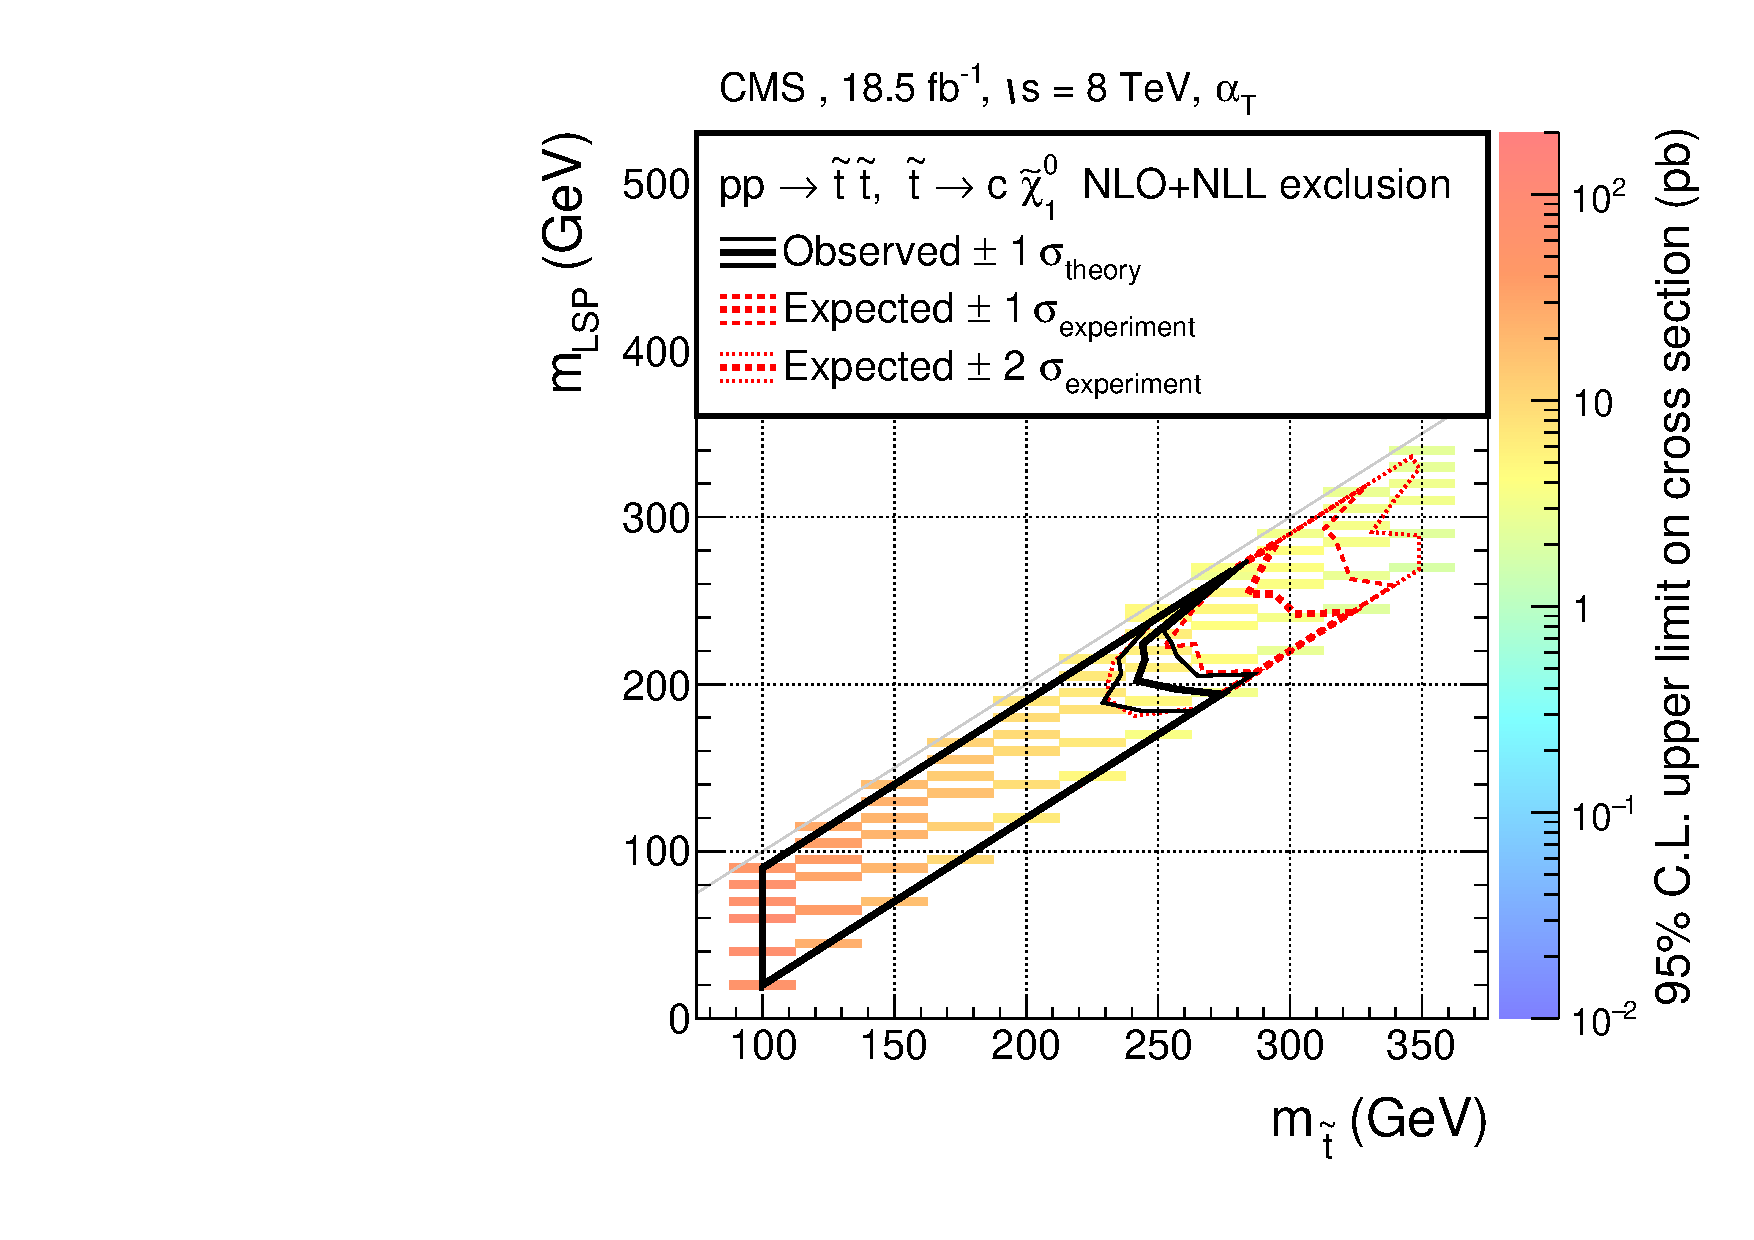
\includegraphics[width=0.44\textwidth]{figures/limits/v3/T2cc_latest_XSEC} 
%    }
%    \subfigure[\label{fig:t24b}${\rm p\bar{p}} \rightarrow \sTop\sTop^{*}, \sTop \rightarrow{\rm bf\bar{f}} \chiz$]{
%      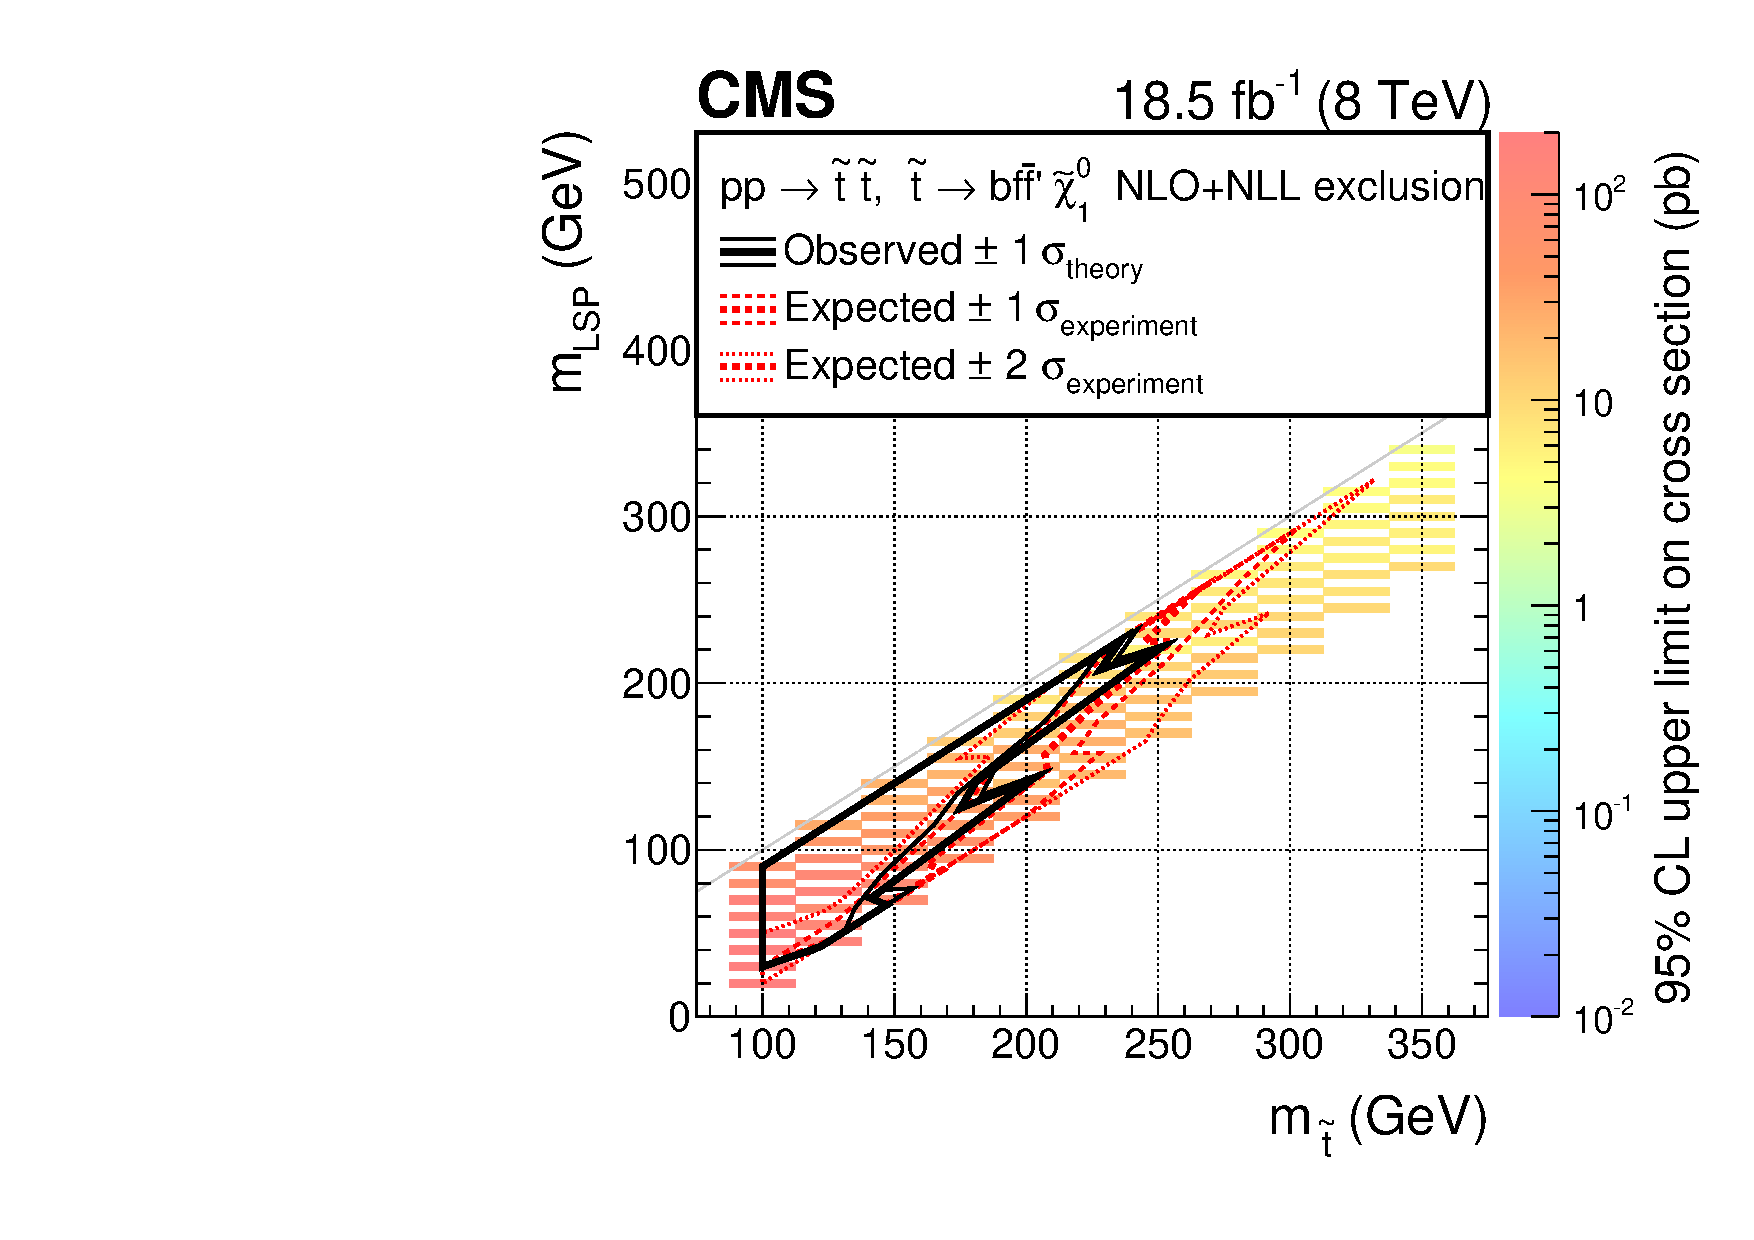
\includegraphics[width=0.44\textwidth]{figures/limits/v3/T2degen_latest_XSEC} 
%    } \\
%\vspace{-0.3cm}
%    \subfigure[\label{fig:t2bw25}${\rm p\bar{p}} \rightarrow  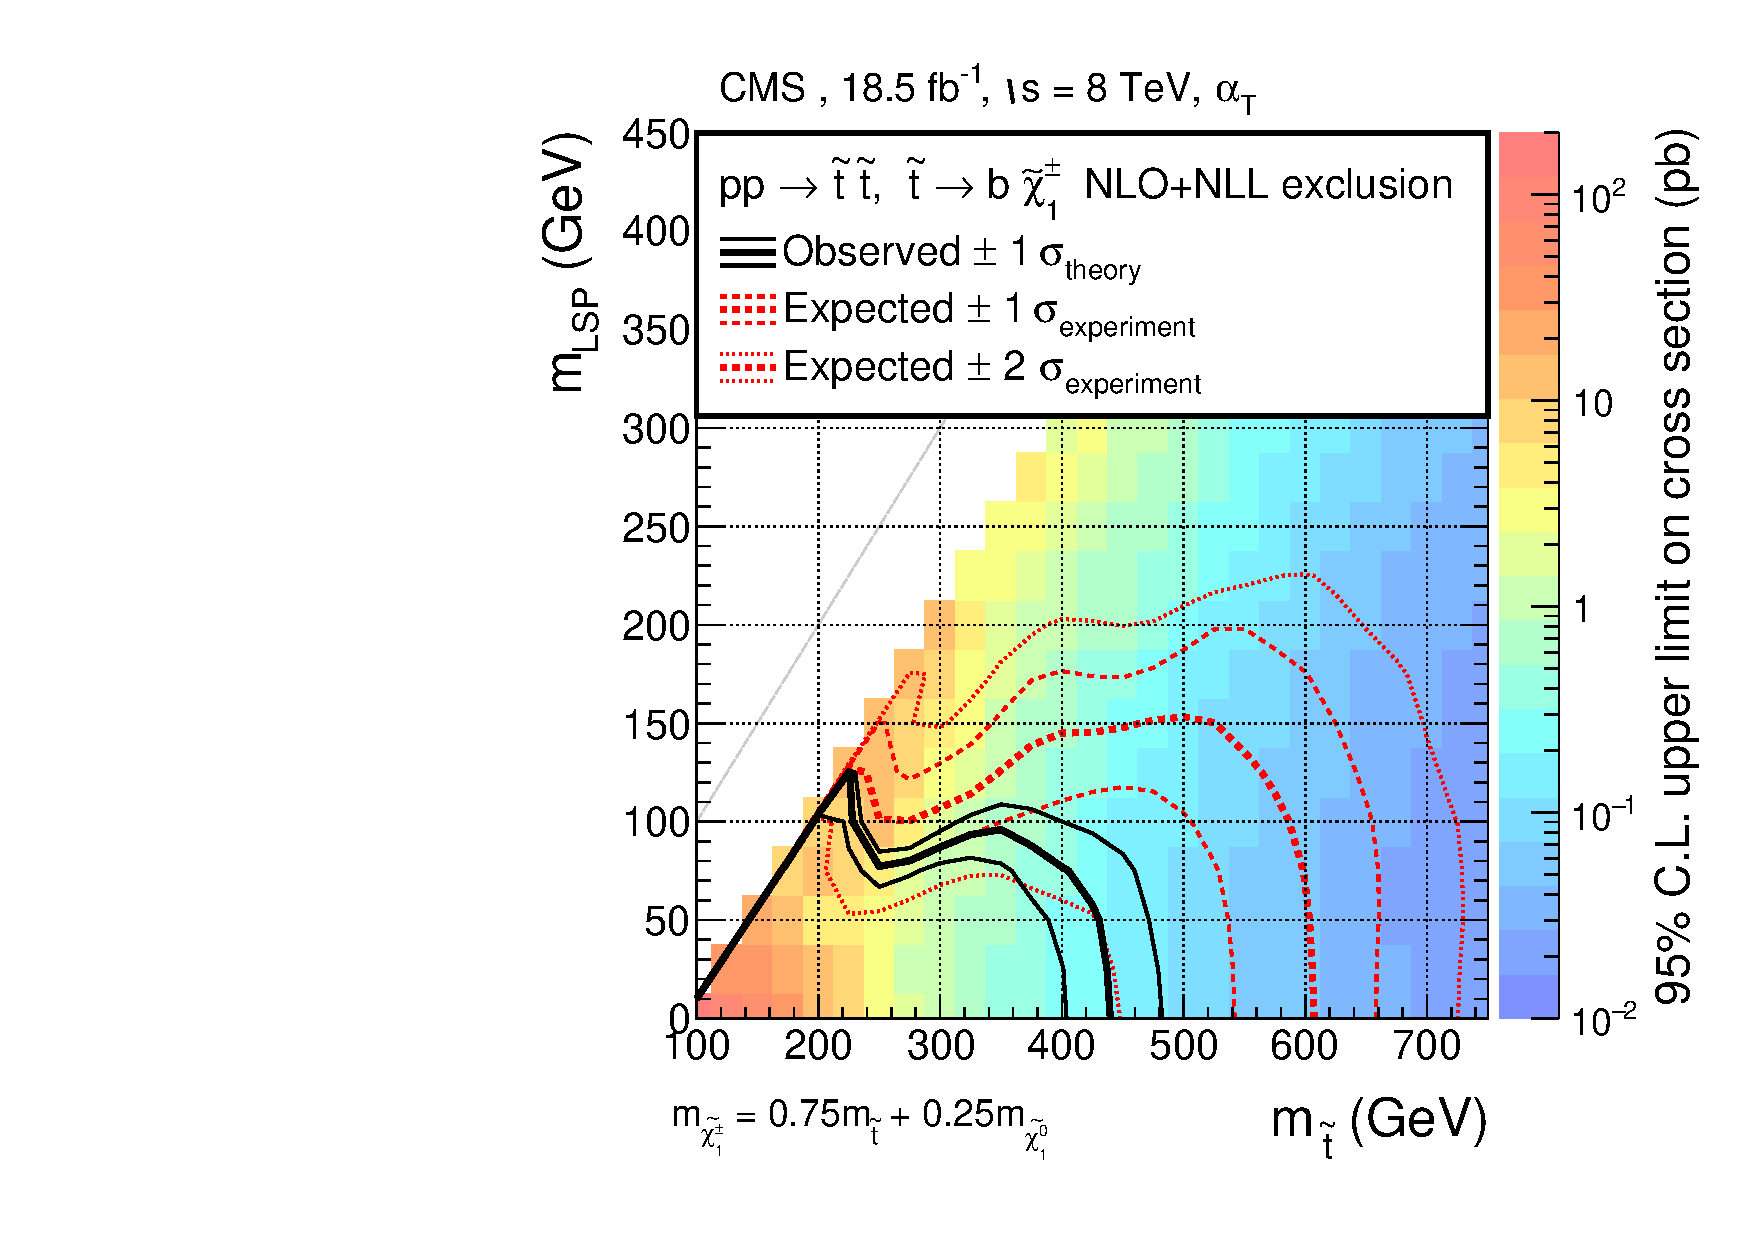
\includegraphics[width=0.44\textwidth]{figures/limits/v4/T2bw0p75_latest_XSEC} 
%    } \\
%\vspace{-0.3cm}
%    \subfigure[\label{fig:t2tt}${\rm p\bar{p}} \rightarrow \sTop\sTop^{*}, \sTop \rightarrow{\rm t} \chiz$]{
%      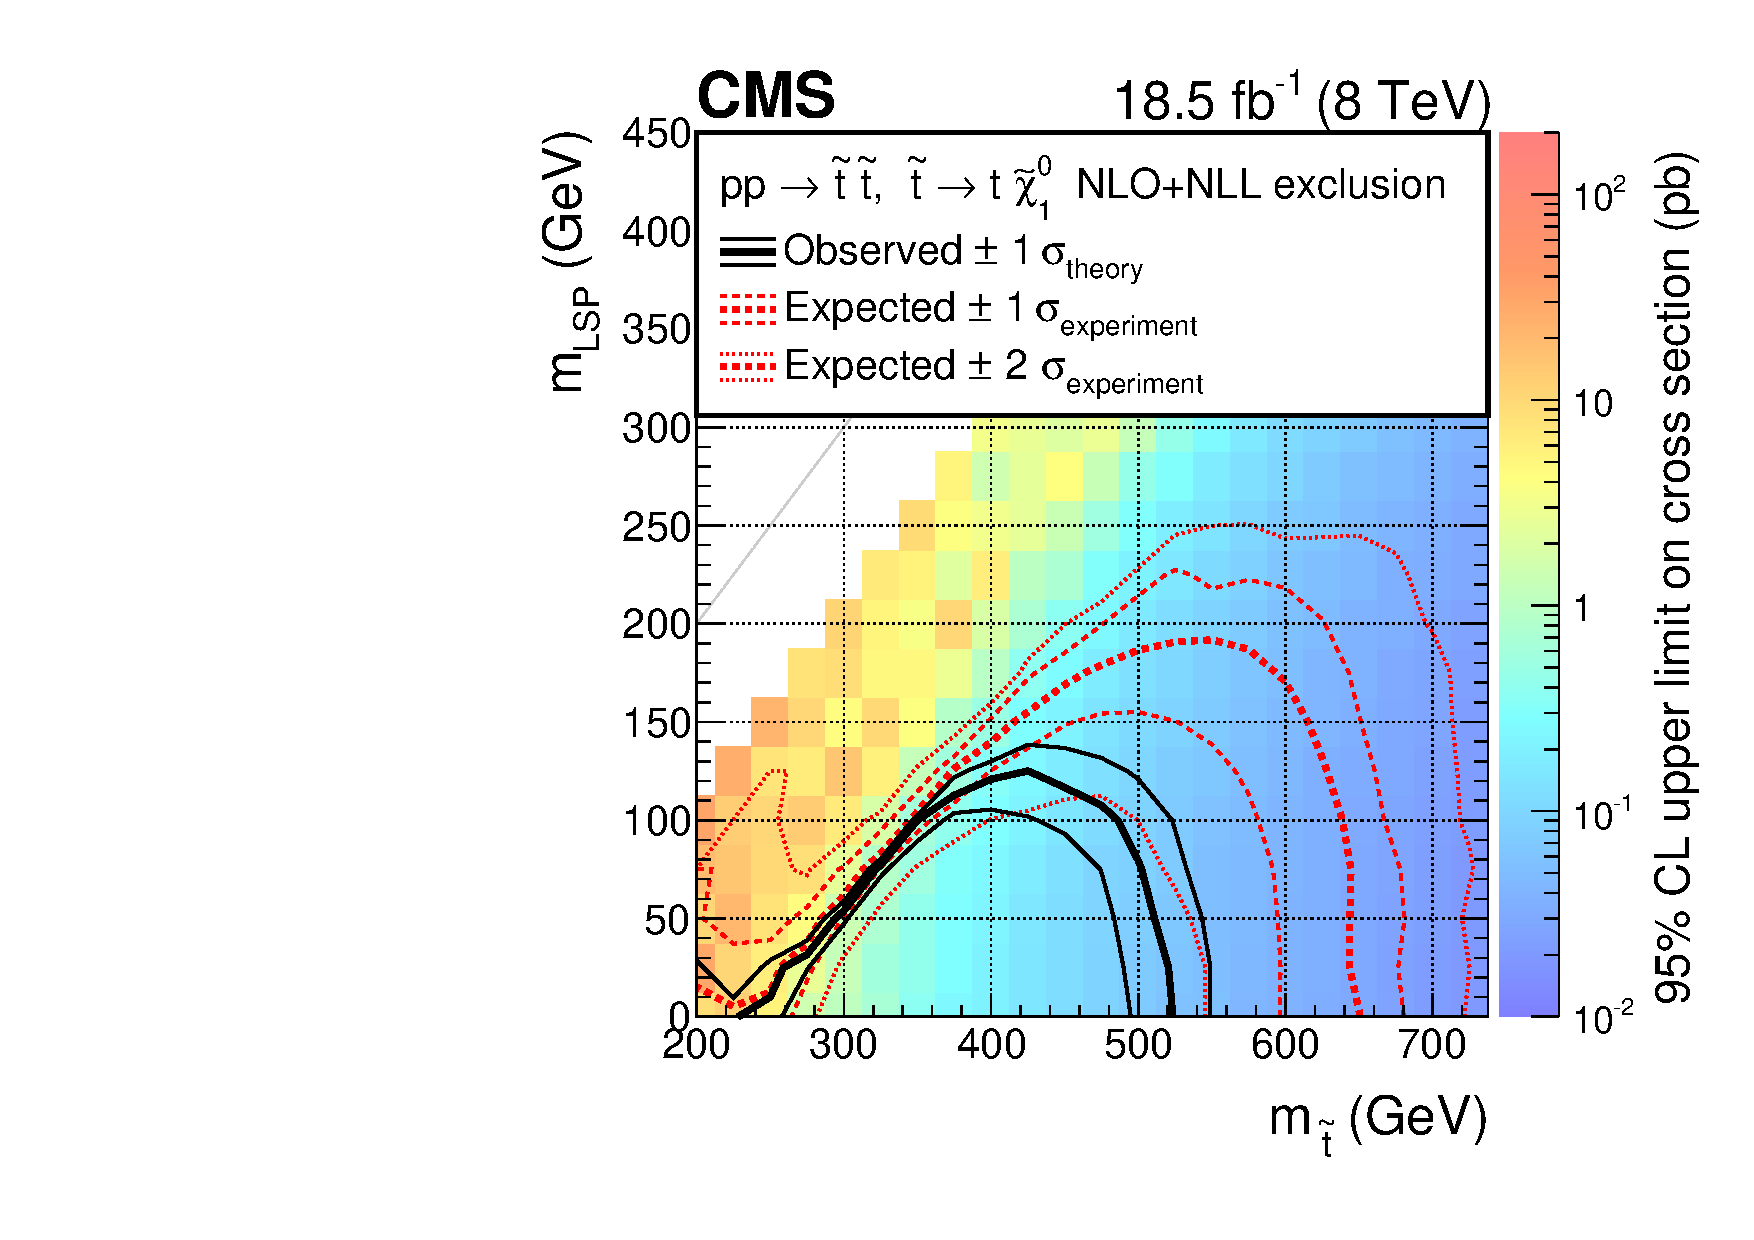
\includegraphics[width=0.44\textwidth]{figures/limits/v4/T2tt_latest_XSEC} 
%    }
%    \subfigure[\label{fig:summary}Summary of expected and observed exclusions.]{
%      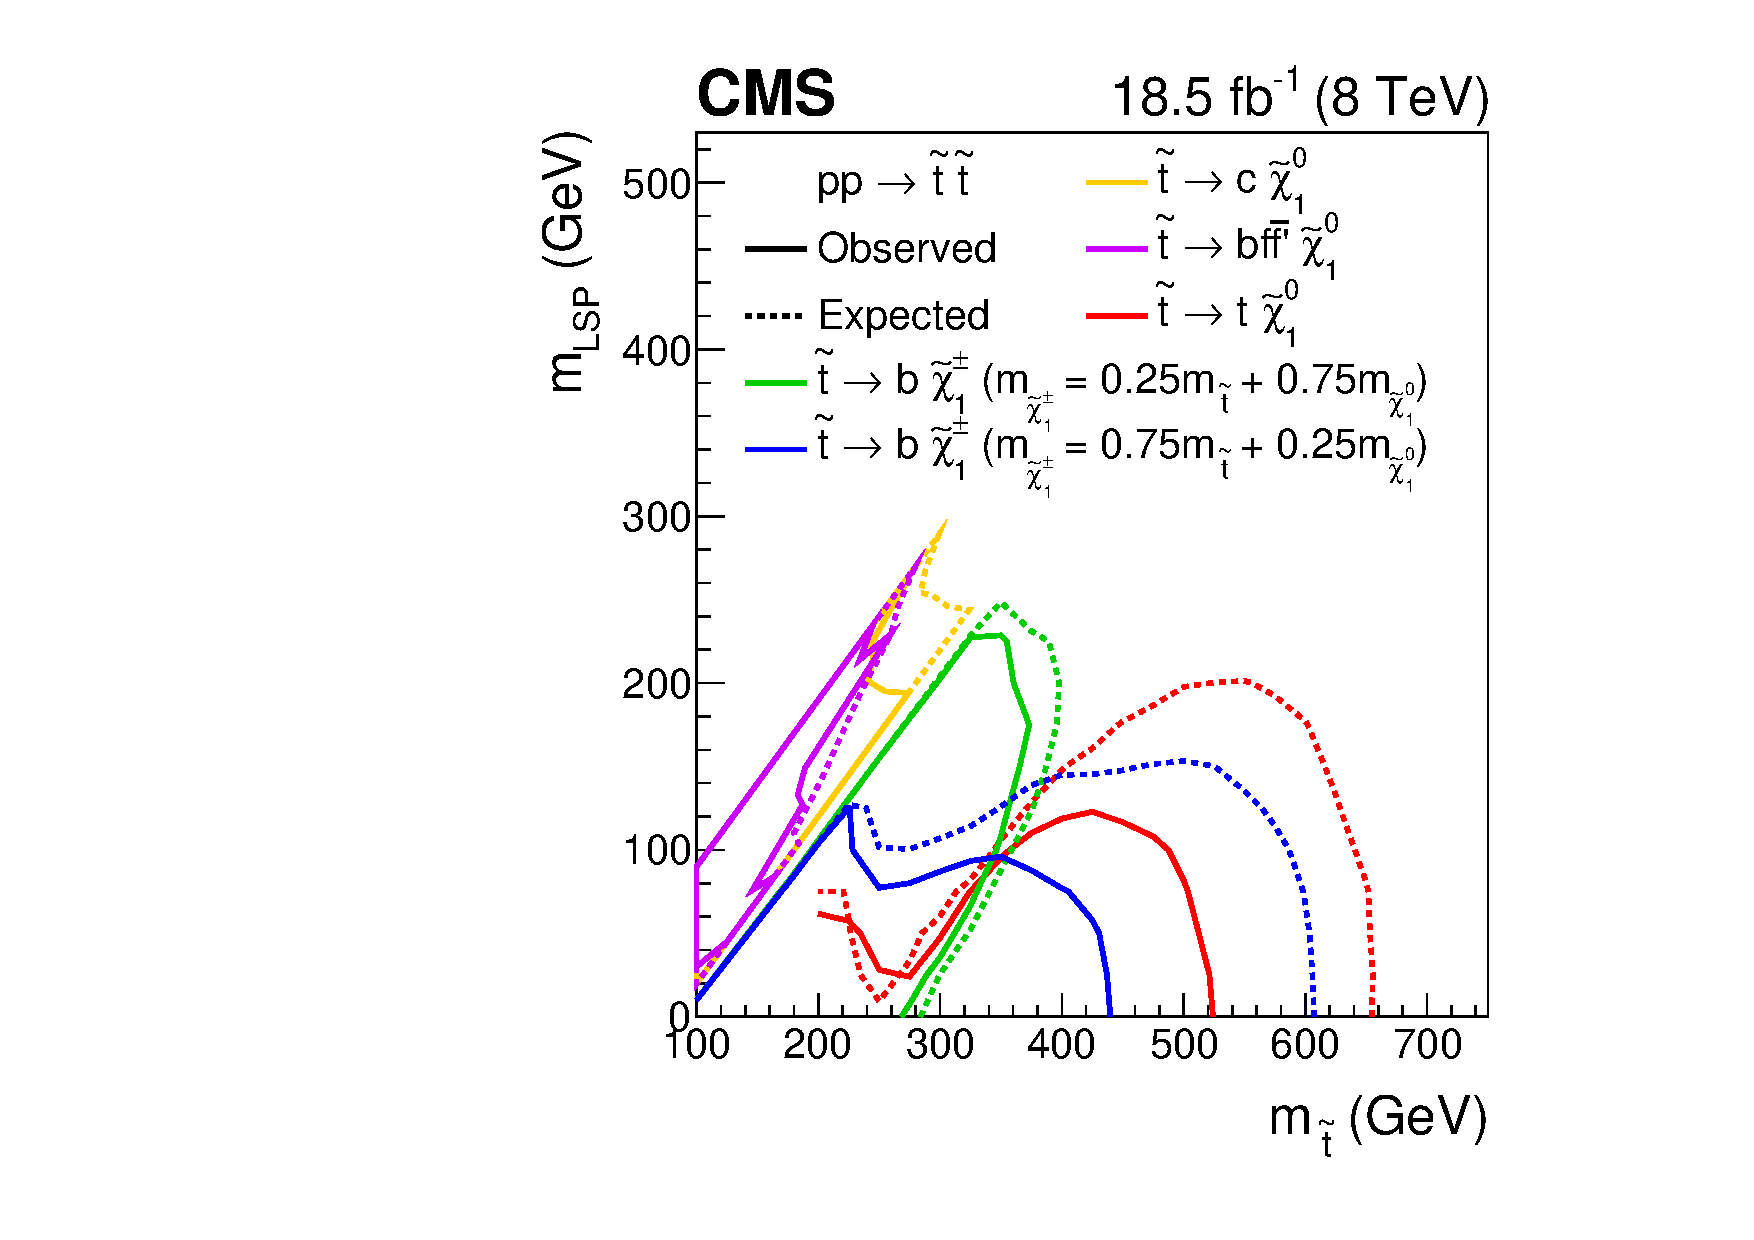
\includegraphics[width=0.44\textwidth]{figures/limits/v4/summary} 
%    } \\
%\vspace{-0.1cm}
%    \caption{ Observed upper limit on the production cross section at 95\% CL (indicated by the colour scale) as a function of the top squark% and $\chiz$ masses for (a) $\sTop \rightarrow{\rm c}
%      \chiz$, (b) $\sTop \rightarrow{\rm bf\bar{f}} \chiz$, (c)
%      $\ black lines reflecting the
%      theoretical uncertainty on the production cross section.
%The black solid thin lines represent the observed exclusions when
%varying the production cross section by its theoretical uncertainty. 
%The red thick dashed (thin dashed
%      or dotted) line indicates the median (${\pm}1 \sigma$ or ${\pm}2
%      \sigma$ experimental uncertainty) expected exclusion.
%Figure (f) shows a summary of the central expected (dotted) and
%observed (solid) exclusions.
%      \label{fig:limits-sms} }
%  \end{center}
%\end{figure*}



Figure~\ref{fig:limits-sms} shows the observed upper limit on the
production cross section at 95\% confidence level (CL) as a function
of the gluino and LSP masses for
a range of simplified models assuming pair production of gluinos. \FIXME{Discuss the limits and put some representative numbers in the test}
%
%
%
%Figures~\ref{fig:t2cc} and~\ref{fig:t24b} show the sensitivity of this
%analysis to the decay modes $\sTop \rightarrow{\rm c} \chiz$ and
% $\sTop \rightarrow{\rm bf\bar{f}} \chiz_1$, respectively. 
The observed excluded regions are determined with NLO+NLL
cross sections for gluino pair production assuming decoupled squarks. Also shown are the
observed excluded regions when varying the production cross section by
its theoretical uncertainty, and the expected excluded region with
both the ${\pm}1$ and ${\pm}2$ standard-deviation ($\sigma$)
variations. 

%The range of excluded top squark masses is sensitive to the both the
%decay mode and $\dm(\sTop,\chiz_1$). For the decay $\sTop \rightarrow{\rm c} \chiz_1$,
%the expected excluded mass region is relatively stable as a function
%of \dm, with masses below 285\gev (325\gev) disfavoured at a 95\% CL
%for $\dm = 0\gev$ ($\dm = 80\gev$). The observed exclusion
%(assuming the theoretical production cross section minus $1\sigma$
%uncertainty) is weaker, with masses below 240\gev (260\gev)
%disfavoured at a 95\% CL for $\dm = 0\gev$ (\dm = 80\gev). 
%For the decay $\sTop \rightarrow{\rm bf\bar{f'}} \chiz_1$, the expected
%excluded mass region is strongly dependent on \dm, weakening
%considerably for increasing values of \dm due to the increased
%momentum phase space available to leptons produced in the 4-body
%decay. Top squark masses below 265\gev (165\gev) are disfavoured with
%a 95\% CL for $\dm = 0\gev$ ($\dm = 80\gev$). The observed exclusion
%is again weaker, with masses below 230\gev (130\gev) disfavoured with
%a 95\% CL for $\dm = 0\gev$ ($\dm = 80\gev$).
%
%Figures~\ref{fig:t2bw25} and~\ref{fig:t2bw75} show the limits on the
%allowed cross section for the decay $\sTop \rightarrow b \chipm_1$,
%followed by a decay of the $\chipm_1$ to $\chiz_1$ plus an on- or off-
%shell W boson, depending on the $\chipm_1 - \chiz_1$ mass difference.
%In these models $x$ indicates the position of the $\chipm_1$ in the mass
%spectrum and its mass is defined as  $m_{\chipm_1} =  x~m_{\sTop} + (1-x)~m_{\chiz_1}$.
%For the case $x$ = 0.25, it can be seen from Figure~\ref{fig:t2bw25} that the analysis has 
%sensitivity in the region $m_{\chipm_1} - m_{\chiz_1} < m_{\rm W}$,
%excluding $\chiz_1$ masses of up to $225 \GeV$ and $\sTop$ masses of
%up to $260 \GeV$.
%In the case of $x$=0.75, $\sTop$ masses of up to $400 \GeV$ can be
%excluded but the reach in $\chiz_1$ mass is reduced.
%Figure~\ref{fig:t2tt} shows the analysis interpretation for the decay
%$\sTop \rightarrow {\rm t} \chiz_1$, where $\sTop$ masses of up to $500 \GeV$ are excluded. 
%As in Figure~\ref{fig:t2bw75}, the
%observed limit is around 2$\sigma$ weaker than the expected for large
%values of $m_{\sTop}$. This is mainly due to an upward fluctuation in data in
%the $\nb=2$ categories in the region $\scalht \sim 500 -700 \GeV$.
%The agreement between observed and expected limits is much better at
%small top squark masses. In this case the signal appears at lower
%values of \scalht where good agreement between data and SM background
%prediction is observed.
%Figure~\ref{fig:summary} shows a summary of all the expected and
%observed exclusions and indicates that the analysis has good
%sensitivity across many different decay signatures in the the $m_{\sTop} - m_{\chiz_1}$ plane.

%The observed mass exclusion regions are marginally weaker than
%expected. The signal best fit point is $m_{\sTop} = X\gev$ and $m_{\rm
%  LSP} = X\gev$ ($m_{\sTop} = X\gev$ and $m_{\rm LSP} = X\gev$) with a
%maximum likelihood value for the signal strength parameter of $\mu =
%1.00 \pm 0.XX$ ($\mu = 1.00 \pm 0.XX$) and a local significance of
%$X\sigma$ ($X\sigma$) for the decay mode $\sTop \rightarrow{\rm c}
%\chiz$ ($\sTop \rightarrow{\rm bf\bar{f}} \chiz$).

%The observed mass exclusion regions are weaker than expected. The
%signal best fit point is $m_{\sTop} = 250\gev$ and $m_{\rm LSP} =
%230\gev$ with a maximum likelihood value for the signal strength
%parameter of $\mu = 1.00 \pm 0.33$, a local significance of
%$3.3\sigma$, and a local p-value of 0.1\%. However, only a subset of
%the signal region bins provide sensitivity to any given model. Hence,
%a look-elsewhere effect must be accounted for when interpreting the
%significance of fluctuations in the data under a specific
%signal+background hypothesis. Given the large number of signal region
%bins and possible SUSY interpretations a trial factor of 10 is
%assumed, resulting in a global p-value and significance of 1\% and
%$2.6\sigma$, respectively.

% The inclusive nature of this search, with signal candidate events
% categorised according to three discriminating variables, ensures
% sensitivity across a range of models. Hence, a global p-value that
% accounts for the look-elsewhere effect will be greater than the
% (local) value quoted above. 
%Assuming $\mathcal{O}(10)$ signal region bins provide the bulk of the
%sensitivity to any given model, a look-elsewhere factor of at least
%$\sim$7 should be assumed, resulting in a global p-value of at least
%$\sim$1\% and a significance of not greater than $\sim2.5\sigma$.}
%Given the large number of signal region bins and possible SUSY
%interpretations a look-elsewhere effect of $\sim$10 is assumed,
%resulting in a global p-value of around 1\% and a significance no
%greater than $2.5\sigma$.

%%__________________________________________________________________||
